
\begin{figure}[!tb]
\centering

\includegraphics[width=0.6\linewidth]{figures/SSDTrain/current_sys_parta_recolored.pdf}
\caption{\label{fig:current_sys} Current clusters and cloud instances usually have limited main memory~\cite{microsoftNDA100V4series2024,googleGPUMachineTypes,ncsaDeltaProjectProfile}.}
\end{figure}

\section{Background and Motivation}

\subsection{GPU Memory Capacity and Model Throughput}
\label{sec:llm_scaling}
As Figure~\ref{fig:eval_dse} of Section~\ref{sec:evaluation} will show, the GPU memory capacity limits the model throughput. By offloading the activations to SSDs, SSDTrain can alleviate this limitation and improve the per-GPU model throughput. An important question is whether the GPU memory capacity will continue to be the limiting factor of per-GPU model throughput according to the trend of LLM scaling. This section shows that the historical trend will make GPU memory capacity an even more critical limiting factor of the per-GPU model throughput.

Neural scaling laws~\cite{jordanhoffmannTrainingComputeOptimalLarge2022,kaplanScalingLawsNeural2020,mccandlishEmpiricalModelLargeBatch2018} guide LLM scaling as computing power increases. We follow these laws in our reasoning.
The whole-system GPU compute throughput $C\propto ND_{batch}$, where $N$ is the number of parameters and $D_{batch}$ is the number of tokens in a batch~\cite{brown2020languagemodelsfewshotlearners}. The Chinchilla scaling law~\cite{jordanhoffmannTrainingComputeOptimalLarge2022} concludes that the optimal model design follows $N\propto C^{0.5}$, which implies $D_{batch}\propto C^{0.5}$ to saturate the GPU throughput.  Whole-system GPU memory use consists of two parts: activations, which require $S_{activations}\propto \frac{N}{h}D_{batch}$, where $h$ is the hidden dimension in the layers and is a slow-growing function of $N$, e.g., $h\propto N^{1/3}$, and all other memory use, $S_{others}\propto N$, including parameters, gradients, and optimizer states. Comparing the factors, we can deduce that (1) $S_{activations}$ grows faster than $S_{others}$, and (2) whole-system memory use, which is dominated by the activations, grows %
slightly slower than the compute throughput $C$ (approximated $C^{5/6}$).
However, Figure~\ref{fig:trend_scale} shows that the historical growth rate of GPU memory capacity (red dotted line) is less than 50\% of that of the compute throughput (yellow dotted line). Therefore, \textbf{GPU memory capacity will become increasingly inadequate for saturating the compute throughput, and memory for activations will continue to dominate the GPU memory usage.} 


What about activation checkpointing? Revisiting the prior equation, $S_{activations}\propto \frac{N}{h}D_{batch}\propto LhD_{batch}$ where $L$ is the number of layers. Activation checkpointing makes the new activations memory use $S_{activations}^\prime \propto \sqrt{L}hD_{batch}$. Since $L$ and $h$ grow when $N$ increases and $D_{batch}\propto C^{0.5}$, $S_{activations}^\prime$ still grows faster than $S_{others}$.

Figure~\ref{fig:main_mem_trend} illustrates the trend of the main memory capacity and Figure~\ref{fig:ssd_trend} illustrates the SSD capacity's trend. As shown, the growth of the main memory capacity still falls behind the demand to sustain GPU throughput growth. On the contrary, the SSD capacity \kwc{better} keeps up with such demand.







\begin{figure}[]
    \centering
    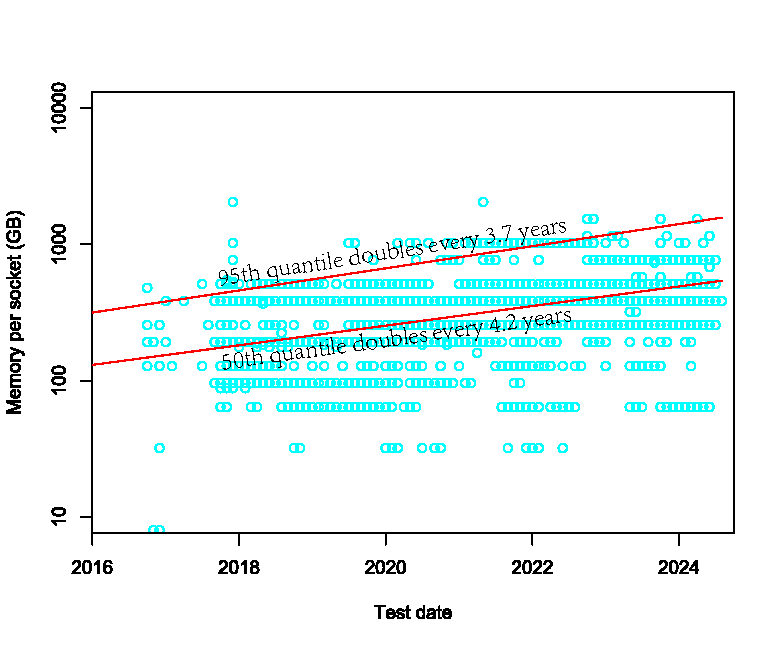
\includegraphics[width=0.8\linewidth]{figures/Intro/MainMemTrend.pdf}
    \caption{The trend of main memory capacity per CPU socket. Data are a dump of all submitted results of SPEC Open System Group (OSG) benchmarks and High-Performance Group (HPG) benchmarks~\cite{specAllSPECOSG2024}. Data points are deduplicated according to (system vendor, system name, CPU model, main memory capacity). Red lines show the growth rates predicted by quantile regression.  The visualization code is adapted from Derek Jones's work~\cite{derekjonesShapeCodeMemory2020}. }
    \label{fig:main_mem_trend}
\end{figure}

\begin{figure}[]
    \centering
    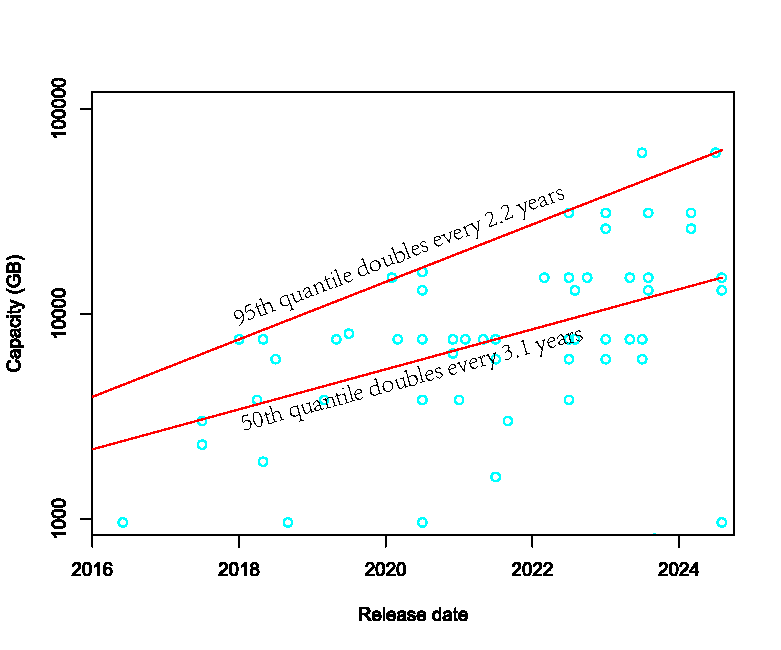
\includegraphics[width=0.8\linewidth]{figures/Intro/SSDTrend.pdf}
    \caption{The trend of enterprise SSD capacity~\cite{techpowerupEnterpriseSSDDatabase2024}. For each model, only the data of the variant with maximal capacity is collected. Red lines show the growth rates predicted by quantile regression.  The visualization code is adapted from Derek Jones's work~\cite{derekjonesShapeCodeMemory2020}. }
    \label{fig:ssd_trend}
\end{figure}



\subsection{SSD Endurance}

Trends in price, latency, and bandwidth have led to the widespread adoption and integration of SSDs into cloud instances and clusters~\cite{microsoftNDA100V4series2024,googleGPUMachineTypes,ncsaDeltaProjectProfile}.
The random write latency of flash has been reduced to tens of microseconds~\cite{samsungUltraLowLatencySamsung2017}, and NVMe SSD data rates are now a few GB/s.


SSD endurance remains a concern: how long will SSDs last in a write-intensive scenario such as activation offloading?
SSD endurance is determined by the type and number of cells, write amplification factor (WAF), and over-provisioning.
SSD cells can be purposed to store one bit, i.e., single-level cells (SLCs), or multiple levels, e.g., triple-level cells (TLCs).
Generally, the more bits a cell stores, the shorter its lifetime in program/erase (P/E) cycles. WAF is the ratio of media write amount to host write amount---SSD writes pages at a time but erases blocks of pages, a coarser granularity. Erasing a partially empty block requires the remaining valid pages to be relocated, causing write amplification. 
In turn, vendors adopt over-provisioning to reserve some blocks for wear leveling, evening out the writes across blocks. 


Table~\ref{tab:ssd} samples current SSD models. The \mbox{D7-P5620} represents a mainstream data center model with 144-layer~(L) TLC cells and a rating of three disk writes per day~(DWPD). The FL6 and \mbox{D7-P5810} SSDs are designed for write-intensive scenarios and have much higher endurance. Notably, SSD endurance rating uses the JESD testing method~\cite{jedecsolidstatetechnologyassociationJESD218BSolidStateDrive2016}, performing random writes after tough preconditioning. In our scenario, the writes are large and sequential, as each tensor being offloaded is easily hundreds of MBs. Such writes are more endurance-friendly than those used to determine the JESD rating. 
For example, \mbox{three-DWPD} SSDs generally allow about 2.5$\times$ as many sequential writes as expected from the JESD rating~\cite{lenovoWhatNeedKnow2023,qnapsystemsinc.QNAPNASSolution2108, smartmodulartechnologiesinc.WhySMARTOverProvisioning2024}. Vendor guidelines~\cite{solidigmSolidigmSSDEndurance,intelOverProvisioningNANDBasedIntel2018,samsungOverProvisioningBenefitsSamsung2019} and empirical data~\cite{maneasOperationalCharacteristicsSSDs2022} corroborate this difference.
Section~\ref{sec:projected_life} conducts modeling to demonstrate why mainstream data center SSDs similar to \mbox{D7-P5620} are viable options to support the deployment of SSDTrain in a large-scale LLM training system.



\begin{table}[!t]
\centering
\begin{tabular}{llll}
\toprule
& \begin{tabular}[c]{@{}l@{}}Kioxia\\ FL6\end{tabular} & \begin{tabular}[c]{@{}l@{}}Solidigm\\ D7-P5620\end{tabular} & \begin{tabular}[c]{@{}l@{}}Solidigm\\ D7-P5810\end{tabular}  \\\midrule
\textbf{3D NAND technology} & 96L SLC & 144L TLC & 144L SLC\\\cline{1-1}
\textbf{\begin{tabular}[c]{@{}l@{}}Endurance rating\\ (DWPD)\end{tabular}}   & 60 & 3 & \begin{tabular}[c]{@{}l@{}}65 (sequential)\\ 50 (random)\end{tabular} \\\cline{1-1}
\textbf{Max capacity} & 3.2 TB & 12.8 TB & 1.6 TB\\\cline{1-1}
\textbf{Max endurance} & 342 PBW  & 65.4 PBW & 146 PBW\\\cline{1-1}
\textbf{Price per PBW} & US\$13.9 & US\$43.8 & US\$11.1\\
\bottomrule
\end{tabular}
\caption{A sample of SSD models in mass production with high endurance in PB writes (PBW)~\cite{solidigmD7P5620MidEndurancePCIe2023,solidigmD7P58102023,neweggSolidigmSolidState2024,kioxiaFL6Series5inch2022,serverorbitKioxiaFL6XHUL1T606TB2024,dihuniSOLIDIGMSSDPF2SQ800GZ01D7P58102024}. \label{tab:ssd}}
\end{table}



\subsection{SSD Offloading Systems for LLM}
\kwc{To offload tensors to SSDs with high performance, SSDTrain utilizes} GPUDirect Storage (GDS)\kwc{, which} enables a direct data path between GPU and local or remote NVMe SSDs~\cite{inupakutikaQuantifyingPerformanceGains2022}. By eliminating the need to involve the CPU for the bounce buffer, \kwc{GDS} enhances bandwidth and reduces both latency and CPU load. 

\kwc{SSDTrain aims to mitigate the training overhead caused by the GPU memory capacity limit, e.g., device underutilization, large pipeline bubble time fraction, etc. In contrast, most existing projects incorporate the offloading mechanism to execute larger models than the original system can fit without offloading at the cost of performance. To this end, there are three differences between SSDTrain and existing work: SSDTrain offloads (a)~activations to (b)~the SSDs (c)~with negligible performance overhead. To the best of our knowledge, SSDTrain is the first work that leverages SSD to offload activations for LLM training.}

\kwc{To take a closer look at the uniqueness of SSDTrain, let us compare it with related work Stronghold}~\cite{sunSTRONGHOLDFastAffordable2022} \kwc{and ZeRO-Infinity}~\cite{rajbhandariZeROinfinityBreakingGPU2021}. \kwc{For difference~(a), SSDTrain offloads activations. Data in LLM training can be categorized into mutually exclusive types: parameters, optimizer states, gradients, and activations.  
In contrast, existing work offloads other data than activations. E.g., Stronghold offloads parameters and gradients. Although ZeRO-Infinity offloads many types of data, when it comes to activations, only a subset as defined in the activation checkpoints, is optionally offloaded.  Activations are the intermediate tensors produced in the forward propagation and kept for gradient computation. They are consumed in the backward propagation immediately after the forward propagation. Due to the high computing cost, gradient computation is best done by GPUs. In comparison, parameter updates associated with parameter and gradient offloading are also light and suitable for CPUs, which is why some work leverages the CPU computing power to update the gradients to improve overall throughput.

For difference~(c), neither ZeRO-Infinity nor Stronghold is designed to hide long data transfer latency. With activation checkpointing in the CPU memory enabled, at the beginning of the backward propagation of each layer, ZeRO-Infinity loads its checkpoint from the CPU memory and waits until it is done. The data transfer latency is in the critical path. Because Stronghold overlaps data transfer with computation, Stronghold’s evaluation performs significantly better than ZeRO-Infinity. Nevertheless, Stronghold  exhibits performance degradation compared with the no-offloading Megatron due to the long transfer latency when using NVMe, as Figures 11 and 14 of Stronghold’s publication show. In contrast, SSDTrain incurs no performance degradation as it overlaps the computation and data transfer well and uses GDS to reduce the SSD access latency.

In summary, SSDTrain must tackle unique challenges, including (i)~the micro-second level SSD latency and (ii)~the short interval between producing activations in the forward propagation and their consumption in the backward propagation. To achieve this, SSDTrain uses GDS to reduce SSD access latency and carefully schedules data movement so that the computation hides the latency.}

Table~\ref{tab:salesman} \kwc{compares the features of} earlier LLM systems supporting \kwc{activation} offloading and SSDTrain:

\noindent
\textbf{Direct GPU--SSD data path.} As Section~\ref{sec:intro} mentions, transfer via CPU interferes with CPU workloads, affecting efficiency. 

\noindent
\textbf{Async data transfer.} These systems either block the training computation when loading the offloaded data or synchronize at each layer. Consequently, the I/O latency is exposed in the critical path. SSDTrain hides the I/O latency by overlapping I/O with GPU computation. 

\noindent
\textbf{Interoperability.} Since LLM training requires a synergy of Python packages and the ecosystem is rapidly evolving, it is vital for the offloading feature to have good interoperability with other components in the same library or other libraries. SSDTrain relies on process-local alternation to PyTorch execution and can work with distributed frameworks, such as Megatron and DeepSpeed. In contrast, DeepSpeed's offloading features, e.g., ZeRO-Infinity, are available only in certain ZeRO stages. \kwc{ZeRO stage determines what is sharded. For example, stage-3 ZeRO in Fig.~\ref{fig:projected_perf_model} sharded optimizer states, gradients, and weights across the data parallel ranks.} Flexgen and LLM in a Flash have their own runtime and do not work with distributed frameworks. 





\begin{table}[!t]
\centering
\begin{tabular}{ @{}l@{\hspace{\tabcolsep}}l@{\hspace{0.5\tabcolsep}}c@{\hspace{0.5\tabcolsep}}c@{\hspace{0.5\tabcolsep}}c@{\hspace{0.5\tabcolsep}}||c@{}}
\toprule
    &       & \rotatebox{68}{Flexgen} & \rotatebox{68}{LLM in a Flash} &\rotatebox{68}{ZeRO-Infinity} & \rotatebox{68}{\textbf{SSDTrain}} \\ 
\midrule  
\multicolumn{2}{@{}l}{\textbf{Training}}                           &           &  & \Checkmark & \Checkmark \\\cline{1-2}
\multirow{2}{*}{\textbf{\begin{tabular}[c]{@{}l@{}}Activation\\ offloading\end{tabular}}}        & \textbf{to main memory}        &    \Checkmark       &  \Checkmark &   Checkpoints only & \Checkmark \\\cline{2-2}
                                   & \textbf{to SSD}          &  \Checkmark         &  &   & \Checkmark \\\cline{1-2}
\multicolumn{2}{@{}l}{\textbf{Direct GPU--SSD data path}}                &           &  &  & \Checkmark\\\cline{1-2}
\multicolumn{2}{@{}l}{\textbf{Async data transfer}}                &           &  &  & \Checkmark\\\cline{1-2}
\multicolumn{2}{@{}l}{\textbf{Interoperability}} & & & & \Checkmark\\
\bottomrule
\end{tabular} 
\caption{Comparing SSDTrain with other LLM systems providing \kwc{activation} offloading features~\cite{shengFlexGenHighThroughputGenerative2023,alizadehLLMFlashEfficient2024,rajbhandariZeROinfinityBreakingGPU2021}. Without backward propagation, inference systems may discard most intermediate tensors once a layer is done. We generalize ``\textbf{Activation}'' to refer to the key-value (KV) cache in inference systems because it is reused across steps. \label{tab:salesman}}
\end{table}
